\documentclass[english,compress]{beamer}
\usepackage{kloeckislides}
\nonstopmode

\usepackage[normalem]{ulem}
\usepackage{pifont}
\usepackage{ifthen}

\setbeamercolor{section in head/foot}{use=structure,bg=structure.fg!25!bg}
\defbeamertemplate*{footline}{split theme}
{%
  \leavevmode%
  \begin{beamercolorbox}[wd=.5\paperwidth,ht=2.5ex,dp=1.125ex]{section in head/foot}%
    \insertsectionnavigationhorizontal{\paperwidth}{\hskip0pt plus1filll}{}%
  \end{beamercolorbox}%
  %\begin{beamercolorbox}[wd=.5\paperwidth,ht=2.5ex,dp=1.125ex]{subsection in head/foot}%
    %\insertsubsectionnavigationhorizontal{.5\paperwidth}{}{\hskip0pt plus1filll}%
  %\end{beamercolorbox}%
}


%\useoutertheme[subsection=false]{miniframes}

\setbeamertemplate{frametitle}[default][center]

\AtBeginDocument{%
  {
    \usebeamercolor{section in head/foot}
  }
  
  \pgfdeclareverticalshading{beamer@headfade}{\paperwidth}
  {%
    color(0cm)=(bg);
    color(1.25cm)=(section in head/foot.bg)%
  }

  \setbeamercolor{section in head/foot}{bg=}
}

\addtoheadtemplate{\pgfuseshading{beamer@headfade}\vskip-1.25cm}{}

\beamertemplatedotitem

\setbeamercolor{section in head/foot}{parent=palette quaternary}
\setbeamercolor{subsection in head/foot}{parent=palette primary}

\setbeamercolor{author in head/foot}{parent=section in head/foot}
\setbeamercolor{title in head/foot}{parent=subsection in head/foot}



\AtBeginSection[] {
  \begin{frame}<beamer>
  \frametitle{Outline}
  \tableofcontents[sectionstyle=show/shaded,subsectionstyle=show/show/hide]
\end{frame}
}
\AtBeginSubsection[] {
  \begin{frame}<beamer>
  \frametitle{Outline}
  \tableofcontents[sectionstyle=show/shaded,subsectionstyle=show/shaded/hide]
\end{frame}
}

\newcommand{\technicality}[2]{%
  {\strut #1\\
    \begin{beamercolorbox}[sep=1mm]{block body}
      #2
    \end{beamercolorbox}
  }%
}

\lstset{
  language=C++,
  rangebeginprefix=//\ ,
  rangeendprefix=//\ ,
}

\def\weblink#1#2{\href{#1}{\color{blue}\underline{#2}}}

\definecolor{fetch}{RGB}{227,110,35}
\definecolor{alu}{RGB}{255,188,24}
\definecolor{context}{RGB}{132,146,175}

\usepackage{keystroke}

\setbeamertemplate{navigation symbols}{}

\def\hilite<#1>#2{\alt<#1>{\colorbox{blue!30}{#2}}{\colorbox{white}{#2}}%
}

\lstset{
  language=C++,
  rangebeginprefix=/*\ ,
  rangeendprefix=/*\ ,
}

\begin{document}
% {{{ front matter

\title{High-Performance Scientific Computing\\Lecture 8: CPU Performance}

\date{MATH-GA 2011 / CSCI-GA 2945 $\cdot$ October 24, 2012}

\frame{\titlepage}

\begin{frame}{Today}
  \tableofcontents[hideallsubsections]
\end{frame}
% }}}
% -----------------------------------------------------------------------------
\begin{frame}{Bits and pieces}
  \begin{itemize}
    \item HW4: \dots
    \item HW6: due Saturday (ask for ext'n early)
    \item Last homework $\rightarrow$ project work after that
    \item Might issue problem sets for entertainment
  \end{itemize}
\end{frame}
% -----------------------------------------------------------------------------
\section[Software]{Tool of the day: Installing software}
% -----------------------------------------------------------------------------
\begin{frame}{Software Installation}
  \begin{center}
  \Huge Demo time
  \end{center}
\end{frame}
% -----------------------------------------------------------------------------
\section{Closer to the machine}
% -----------------------------------------------------------------------------
\def\procpic{
  \node [rectangle,draw,thick,fill=green!30, inner xsep=4cm,
    anchor=south] at (0,0) (idbus) { Internal Bus };
  \node (reg) [rectangle,draw,thick,fill=black!20,
    inner ysep=5mm,anchor=south]
    at ($ (idbus.north) + (-2cm,0.75) $) {Register File} ;
  \node (flags) [anchor=south east,draw,thick,fill=black!20,inner ysep=0.75mm]
    at(reg.south east) {Flags} ;
  \node (alu) [trapezium,
    trapezium left angle=130,
    trapezium right angle=130,
    inner ysep=3mm,
    draw,thick,fill=black!20,anchor=north]
    at ($ (idbus.south) + (2,-0.75) $) {Data ALU} ;
  \node (addr) [trapezium,
    trapezium left angle=50,
    trapezium right angle=50,
    inner ysep=3mm,
    draw,thick,fill=black!20,anchor=south west]
    at ($ (reg.north) + (0,0.75) $) {Address ALU} ;
  \node (ctrl) [arrow box,draw,thick,fill=black!20,anchor=north,
    inner ysep=5mm,arrow box arrows={north:.475cm,east:.475cm},
    arrow box shaft width=2mm,inner xsep=4mm]
    at ($ (idbus.south) + (-2cm,-0.275) $) {Control Unit} ;
  \node (pc) [anchor=north east,draw,thick,fill=black!20,inner ysep=0.75mm]
    at(ctrl.north east) {PC} ;
  \node (mem) [rectangle,draw,thick,fill=black!20,
    inner ysep=3mm,anchor=west,rotate=90,inner xsep=5mm,minimum
    width=3.5cm, minimum height=1cm]
    at ($ (idbus.north) + (2,0.75) $) { } ;
  \node at (mem.south east) [anchor=north west] {Memory Interface} ;
  \draw [line width=1mm,<-] (alu.north west) -- +(0,0.75) ;
  \draw [line width=1mm,<-] (alu.north east) -- +(0,0.75) ;
  \draw [line width=1mm,->] (alu.south) |- +(1,-0.25) -| ($ (idbus.south) + (4.5,0) $);
  \draw [line width=1mm,<->] (reg.south) -- +(0,-0.75);
  \draw [line width=1mm,->] (reg.north) -- (addr.south west);
  \draw [line width=1mm,->] ($ (idbus.north) + (-0.5,0) $) |- ++(0,2.5) -| (addr.south east);
  \draw [line width=1mm,->] ($ (idbus.south) + (-4,0) $) |- (ctrl.west)
    node [pos=0.3,anchor=east,font=\footnotesize,text width=7mm] {Insn. fetch};
  \draw [line width=1mm,->] (addr.north) |- ++(2.6,0.25) |- (mem.north) ;
  \draw [line width=1mm,<->] (mem.west) -- +(0,-0.75) ;
  \draw [line width=1mm,<->] (mem.west) -- +(0,-0.75) ;
  \draw [line width=1mm,<->] (mem.west) -- +(0,-0.75) ;
  \draw [line width=1mm,<->] ($ (mem.south) + (0,-.75) $) coordinate (dataexit) -- +(0.75,0)
    node [pos=1,anchor=west] {Data Bus} ;
  \draw [line width=1mm,->] ($ (mem.south) + (0,.75) $) coordinate (addrexit) -- +(0.75,0)
    node [pos=1,anchor=west] {Address Bus} ;

  \draw [line width=1mm,dotted,opacity=0.3] (dataexit) -| (mem.west) ;
  \draw [line width=1mm,dotted,opacity=0.3] (addrexit) -| ++(-0.4,0) |- (mem.north) ;
}
\begin{frame}{A Basic Processor}
  \begin{tikzpicture}
    \procpic
  \end{tikzpicture}
  {\small (loosely based on Intel 8086)}
  \uncover<2>{
    \begin{tikzpicture} [overlay]
      \node [draw,drop shadow,fill=white,anchor=south west,xshift=1cm,yshift=1.5cm,
      text width=0.4\textwidth, inner xsep=0.5cm,inner ysep=0.5cm,thick]
        at (current page.south west)
        {
        \emph{Bonus Question:}

        What's a
        \weblink{http://en.wikipedia.org/wiki/Bus_(computing)}{bus}?
        } ;
    \end{tikzpicture}
  }
\end{frame}

% -----------------------------------------------------------------------------
\subsection[Assembly]{Machine Language}
% -----------------------------------------------------------------------------
% {{{
\begin{frame}[fragile]{A Very Simple Program}
  \begin{columns}
    \column{0.25\textwidth}
    \lstinputlisting[linerange=start-end]{assembly.c}
    \column{0.75\textwidth}
    \lstinputlisting[language=HTML,basicstyle=\footnotesize]{assembly.S}
  \end{columns}

  Things to know:
  \begin{itemize}
  \item \weblink{http://en.wikipedia.org/wiki/Addressing_mode}{Addressing
  modes} (Immediate, Register, Base plus Offset)
  \item
  \weblink{http://en.wikipedia.org/wiki/Hexadecimal}{0xHexadecimal}
  \item ``AT\&T Form'': (we'll use this)\\
    \verb|<opcode><size> <source>, <dest>|
  \end{itemize}
\end{frame}
\begin{frame}{Another Look}
  \begin{tikzpicture}
    \procpic
  \end{tikzpicture}
  \uncover<2>{
  \begin{tikzpicture} [overlay]
    \node [draw,drop shadow,fill=white,anchor=north east,xshift=-0.5cm,yshift=-0.5cm,
    text width=0.6\textwidth, inner ysep=1mm,thick,inner xsep=3mm]
      at (current page.north east)
      {
        \lstinputlisting[language=HTML,basicstyle=\tiny]{assembly.S}
      } ;
  \end{tikzpicture}
  }
\end{frame}
\begin{frame}[fragile]{A Very Simple Program: Intel Form}
  \lstinputlisting[language=HTML,basicstyle=\footnotesize]{assembly-intel.S}

  \begin{itemize}
  \item ``Intel Form'': (you might see this on the net)\\
    \verb|<opcode> <sized dest>, <sized source>|
  \item Goal: Reading comprehension.
  \item Don't understand an opcode?\\
    Google ``\verb|<opcode> intel instruction|''.
  \end{itemize}
\end{frame}
\begin{frame}{Machine Language Loops}
  \begin{columns}
    \column{0.3\textwidth}
    \lstinputlisting{loop-assembly.c}
    \column{0.75\textwidth}
    \lstinputlisting[language=HTML,basicstyle=\scriptsize]{loop-assembly.S}
  \end{columns}

  Things to know:
  \begin{itemize}
  \item
  \weblink{http://en.wikipedia.org/wiki/Status_register}{Condition
  Codes (Flags)}: Zero, Sign, Carry, etc.
  \item \weblink{http://en.wikipedia.org/wiki/Call_stack}{Call Stack}:
    Stack frame, stack pointer, base pointer
  \item
  \weblink{http://en.wikipedia.org/wiki/Application_binary_interface}{ABI}:
    Calling conventions
  \end{itemize}
\end{frame}
% -----------------------------------------------------------------------------
\begin{frame}{Web demo}
  \begin{center}
  \Huge \url{http://assembly.ynh.io/} demo time
  \end{center}
\end{frame}
% -----------------------------------------------------------------------------
\begin{frame}{Other web-based assembly viewers}
  \begin{itemize}
    \item \url{http://assembly.ynh.io/}

      [\url{https://github.com/ynh/cpp-to-assembly}]
    \item \url{http://gcc.godbolt.org/}

    \item \url{http://llvm.org/demo/}
  \end{itemize}
\end{frame}
% -----------------------------------------------------------------------------
\begin{frame}{DIY demo}
  \begin{center}
  \Huge Assembly comprehension/optimizer
  \end{center}
\end{frame}
% }}}
% -----------------------------------------------------------------------------
\subsection{Memory}
% -----------------------------------------------------------------------------
% {{{
\begin{frame}{What is\dots a Memory Interface?}
  \begin{columns}
    \column{0.7\textwidth}
      \textbf{Memory Interface} gets and stores binary words in
      off-chip memory.
      \medskip

      Smallest granularity: Bus width
      \medskip

      Tells outside memory
      \begin{itemize}
        \item ``where'' through \emph{address bus}
        \item ``what'' through \emph{data bus}
      \end{itemize}

      Computer main memory is ``Dynamic RAM''
      (\weblink{http://en.wikipedia.org/wiki/Dynamic_random_access_memory}{DRAM}):
      Slow, but small and cheap.

    \column{0.3\textwidth}
      \includegraphics[width=\textwidth]{memory.png}
  \end{columns}
\end{frame}
\input{how-does-computer-memory-work}
\begin{frame}{DRAM}
  \begin{center}
    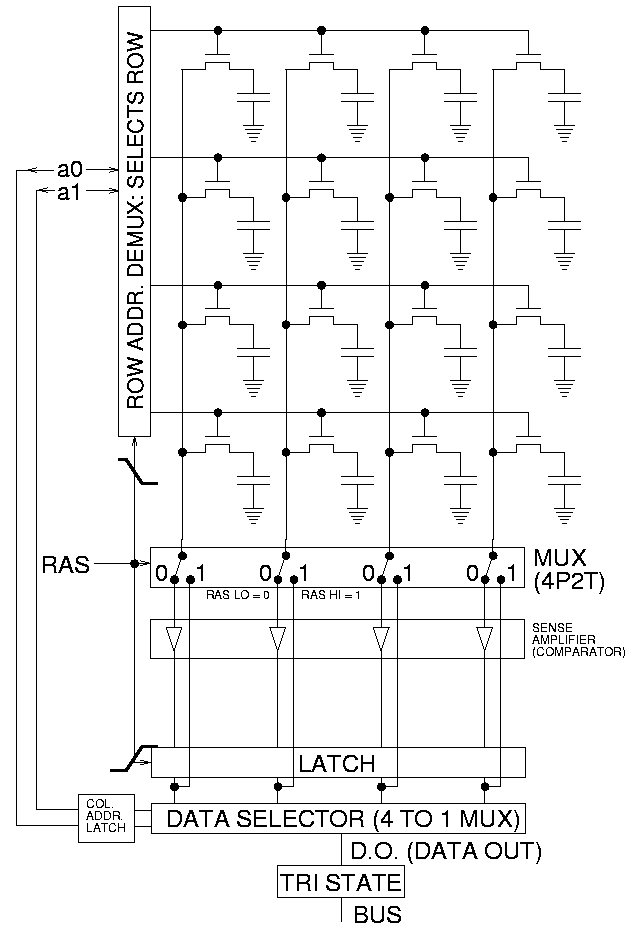
\includegraphics[height=7cm]{dram.png}
  \end{center}
  \uncover<2>{
    \begin{tikzpicture} [overlay]
      \node [above left=1cm of current page.south east,draw,drop shadow,fill=white,
       inner sep=5mm,thick]
        {
          Key: each cell is \emph{tiny} $\rightarrow$ many of them!
        } ;
    \end{tikzpicture}
  }
\end{frame}
\addimgcredit{DRAM: Wikipedia \cc}
% -----------------------------------------------------------------------------
\begin{frame}{DRAM die}
  \begin{center}
    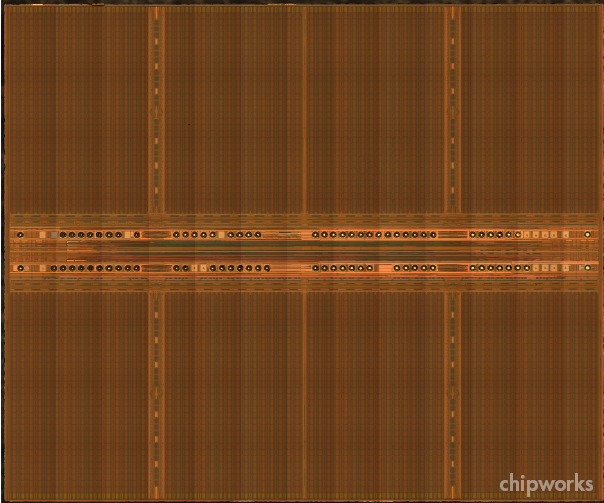
\includegraphics[height=7cm]{dram-die.png}

    \medskip
    Samsung 1 Gib DDR3 die
  \end{center}
\end{frame}
\addimgcredit{DRAM die: chipworksrealchips.com / Samsung}
% -----------------------------------------------------------------------------
\section[Faster]{Making things go faster}
% -----------------------------------------------------------------------------
\subsection{Overview}
% -----------------------------------------------------------------------------
\begin{frame}{We know how a computer works!}

  All of this can be built in about 4000 transistors.

  (e.g. MOS 6502 in Apple II, Commodore 64, Atari 2600)
  \medskip

  So what exactly is Intel doing with the other 623,996,000 transistors?
  \medskip

  Answer: \uncover<2->{\emph{Make things go faster!}}
  \medskip

  \uncover<3->{
  \textbf{Goal now:}

  Understand sources of slowness, and how they get addressed.
  \medskip

  Remember: \emph{High Performance} Computing
  }
\end{frame}
% -----------------------------------------------------------------------------
\subsection[Memory]{The Memory Hierarchy}
% -----------------------------------------------------------------------------
\begin{frame}{Source of Slowness: Memory}
  Memory is slow.
  \medskip

  Distinguish two different versions of ``slow'':
  \begin{itemize}
    \item Bandwidth
    \item Latency
  \end{itemize}
  $\rightarrow$ Memory has \emph{long latency}, but can have
  \emph{large bandwidth}.

  \begin{center}
  \includegraphics[width=0.4\textwidth]{mainboard.jpeg}
  \end{center}

  Size of die vs. distance to memory: big!

  \medskip
  Dynamic RAM: long intrinsic latency!

  \uncover<2>{
    \begin{tikzpicture} [overlay]
      \node [draw,drop shadow,fill=white,anchor=south east,xshift=-0.5cm,yshift=0.5cm,
      text width=0.4\textwidth, inner sep=3mm,thick]
        at (current page.south east)
        {
        \emph{Idea:}\\[1ex]
        Put a look-up table of recently-used data onto the
        chip.\\[1ex]
        $\rightarrow$
        ``\weblink{http://en.wikipedia.org/wiki/CPU_cache}{Cache}''
        } ;
    \end{tikzpicture}
  }
\end{frame}

% -----------------------------------------------------------------------------
\begin{frame}{The Memory Hierarchy}
  Hierarchy of increasingly bigger, slower memories:

  \begin{center}
  \begin{tikzpicture}[hieblock/.style={thick,draw,fill=green!20,
  text width=0.4\textwidth, text centered}]
    \node [hieblock] (reg) {Registers};
    \node [hieblock,below=3ex of reg] (l1) {L1 Cache};
    \node [hieblock,below=3ex of l1] (l2) {L2 Cache};
    \node [hieblock,below=3ex of l2] (dram) {DRAM};
    \node [hieblock,below=3ex of dram] (virt) {Virtual Memory\\ (hard drive)};

    \node [right=2em of reg] {1 kB, 1 cycle };
    \node [right=2em of l1] {10 kB, 10 cycles };
    \node [right=2em of l2] {1 MB, 100 cycles };
    \node [right=2em of dram] {1 GB, 1000 cycles };
    \node [right=2em of virt] {1 TB, 1 M cycles };

    \draw [thick,<->] (reg) -- (l1) ;
    \draw [thick,<->] (l1) -- (l2) ;
    \draw [thick,<->] (l2) -- (dram) ;
    \draw [thick,<->] (dram) -- (virt) ;
  \end{tikzpicture}
  \end{center}
  \uncover<2>{
    \begin{tikzpicture} [overlay]
      \node [draw,drop shadow,fill=white,anchor=south east,xshift=-0.5cm,yshift=0.5cm,
      text width=0.6\textwidth, inner sep=5mm,thick]
        at (current page.south east)
        {
          Second red/blue pebble game: played by cache controller

          \bigskip
          What is a \emph{working set}?

          \bigskip
          How might \emph{data locality} factor into this?
        } ;
    \end{tikzpicture}
  }
\end{frame}

% -----------------------------------------------------------------------------
\begin{frame}{Cache: Actual Implementation}
  \begin{columns}
    \column{0.55\textwidth}
      Demands on cache implementation:
      \begin{itemize}
        \item Fast, small, cheap, low power
        \item Fine-grained
        \item High ``hit''-rate (few ``misses'')
      \end{itemize}

    \column{0.4\textwidth}
      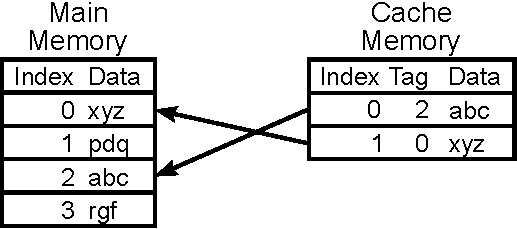
\includegraphics[width=\textwidth]{basic-cache.pdf}
  \end{columns}

  \bigskip
  \emph{Problem:}

  \colorbox{gray!20}{
  Goals at odds with each other:
  Access matching logic expensive!
  }

  \bigskip
  \emph{Solution 1}: More data per unit of access matching logic\\
  \hfill $\rightarrow$ Larger ``Cache Lines''

  \bigskip
  \emph{Solution 2}: Simpler/less access matching logic\\
  \hfill $\rightarrow$ Less than full ``Associativity''

  \bigskip
  Other choices: Eviction strategy, size
\end{frame}
\addimgcredit{Basic cache: Wikipedia \cc}
% -----------------------------------------------------------------------------
\begin{frame}{Cache: Associativity}
  \begin{center}
    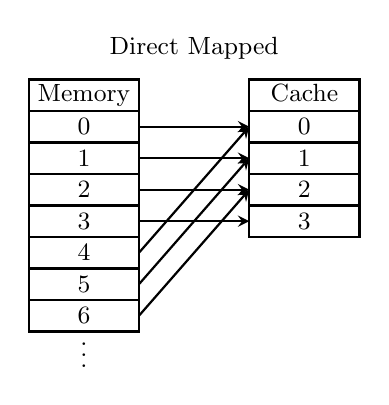
\begin{tikzpicture}[yscale=-0.4,xscale=0.7,font=\small]

      \node at (3,-2) { Direct Mapped } ;
      \draw [thick] (0,0) rectangle +(2,-1)
        node [pos=0.5,text depth=0.4ex] {Memory};
      \foreach\i in {0,1,2,...,6}
      {
        \draw [thick] (0,\i) rectangle +(2,1) node [pos=0.5] {\i};
        \pgfmathtruncatemacro{\tgt}{mod(\i,4)}
        \draw [-stealth,thick] (2,\i+0.5) -- (4,\tgt+0.5) ;
      }
      \node at (1,7.5) { $\vdots$ };

      \draw [thick] (4,0) rectangle +(2,-1)
        node [pos=0.5,text depth=0.4ex] {Cache};
      \foreach\i in {0,1,2,...,3}
      \draw [thick] (4,\i) rectangle +(2,1) node [pos=0.5] {\i};

    \end{tikzpicture}
    \hspace{1cm}
    \uncover<+->{}
    \uncover<+->{
      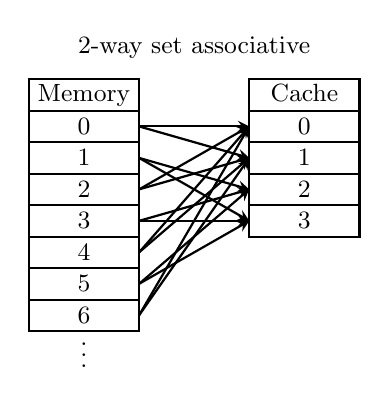
\begin{tikzpicture}[yscale=-0.4,xscale=0.7,font=\small]
        \node at (3,-2) { 2-way set associative } ;
        \draw [thick] (0,0) rectangle +(2,-1)
        node [pos=0.5,text depth=0.4ex] {Memory};
        \foreach\i in {0,1,2,...,6}
        {
          \draw [thick] (0,\i) rectangle +(2,1) node [pos=0.5] {\i};
          \pgfmathtruncatemacro{\tgt}{mod(2*\i,4)}
          \draw [-stealth,thick] (2,\i+0.5) -- (4,\tgt+0.5) ;
          \uncover<+->{
            \pgfmathtruncatemacro{\tgt}{mod(2*\i+1,4)}
            \draw [-stealth,thick] (2,\i+0.5) -- (4,\tgt+0.5) ;
          }
        }
        \node at (1,7.5) { $\vdots$ };

        \draw [thick] (4,0) rectangle +(2,-1)
        node [pos=0.5,text depth=0.4ex] {Cache};
        \foreach\i in {0,1,2,...,3}
        \draw [thick] (4,\i) rectangle +(2,1) node [pos=0.5] {\i};

      \end{tikzpicture}
    }
  \end{center}
  \uncover<+>{
  \begin{tikzpicture} [overlay]
    \node [draw,drop shadow,fill=white,anchor=south east,xshift=-1cm,yshift=1cm,
    text width=0.7\textwidth,thick,inner sep=5mm]
      at (current page.south east)
      {
        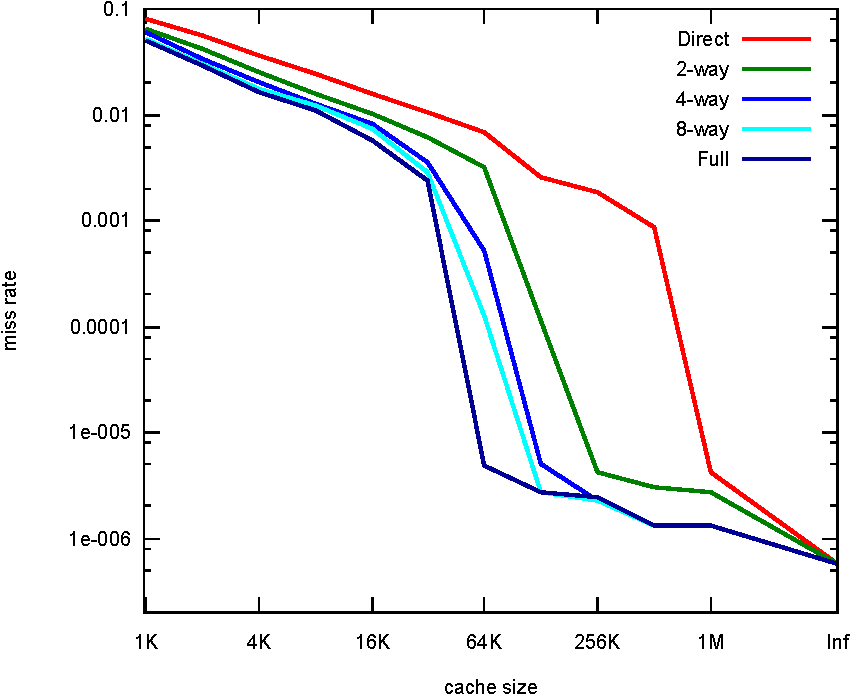
\includegraphics[width=\textwidth]{cache-assoc-miss.pdf}

        Miss rate versus cache size on the Integer portion of
        SPEC~CPU2000 [Cantin, Hill 2003]
      } ;
  \end{tikzpicture}
  }
\end{frame}
\addimgcredit{Cache associativity: based on Wikipedia \cc}
\addimgcredit{Cache associativity vs miss rate: Wikipedia \cc, }

% -----------------------------------------------------------------------------
\begin{frame}{CPUID}
  \begin{center}
  \Huge CPUID demo time
  \end{center}
\end{frame}

\def\cacheslide#1#2{
\begin{frame}{#1}
  \lstinputlisting[basicstyle=\scriptsize]{microbench/#2.c}
  \creditto{Original benchmarks by Igor Ostrovsky}
  \uncover<2>{
    \begin{tikzpicture} [overlay]
      \node [draw,drop shadow,fill=white,anchor=south east,xshift=-0.5cm,yshift=0.5cm,
      text width=0.8\textwidth, inner sep=5mm,thick]
        at (current page.south east)
        {
        \includegraphics[width=\textwidth]{microbench/#2-crop.pdf}
        } ;
    \end{tikzpicture}
  }
\end{frame}
}

\cacheslide{Updating every $k$th integer}{strides}
\cacheslide{Measuring bandwidths}{bw}
\cacheslide{Another mystery}{assoc}

\addimgcredit{Cache Measurements: Igor Ostrovsky}

% -----------------------------------------------------------------------------
\begin{frame}{Core Message}
  \begin{center}
    Learned a lot about caches.

    \bigskip
    Also learned:

    \bigskip
    {\Large Honest measurements are \emph{hard}.}

    \vspace{2cm}
    A good attempt:

    \url{http://www.bitmover.com/lmbench/}

    \footnotesize
    Instructions:

    \url{http://download.intel.com/design/intarch/papers/321074.pdf}
  \end{center}
\end{frame}
% -----------------------------------------------------------------------------
\begin{frame}{Programming for the Hierarchy}
  How can we rearrange programs to friendly to the memory hierarchy?

  \bigskip
  Examples:
  \begin{itemize}
  \item<+-> Large vectors $x$, $a$, $b$

  Compute\[
  x \leftarrow x+3a-5b.
  \]
  \item<+-> Matrix-Matrix Multiplication
  \end{itemize}
\end{frame}
% }}}
% -----------------------------------------------------------------------------
\subsection{Pipelines}
% -----------------------------------------------------------------------------
% {{{
\begin{frame}{Source of Slowness: Sequential Operation}
  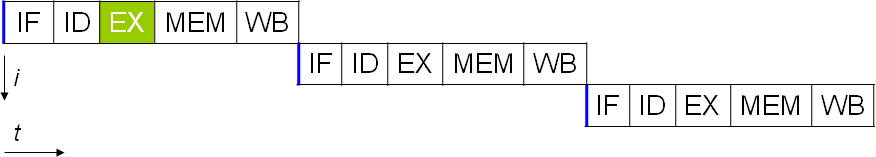
\includegraphics[width=\textwidth]{no-pipeline.png}
  \begin{description}
    \item[IF] Instruction fetch
    \item[ID] Instruction Decode
    \item[EX] Execution
    \item[MEM] Memory Read/Write
    \item[WB] Result Writeback
  \end{description}
\end{frame}
\addimgcredit{Pipelining: Wikipedia \cc}
\begin{frame}{Solution: Pipelining}
  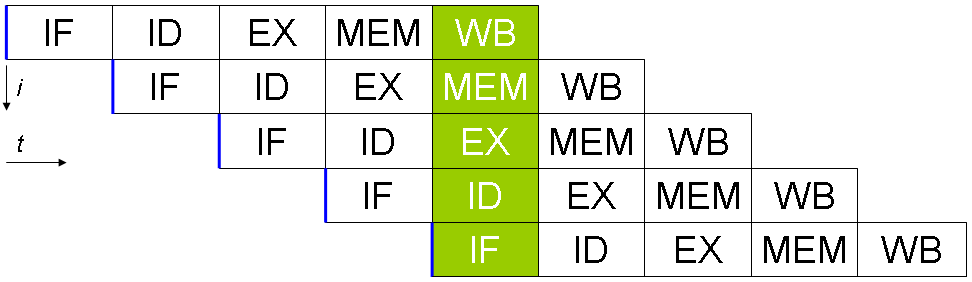
\includegraphics[width=\textwidth]{five-stage-pipeline.png}
\end{frame}
\begin{frame}{Pipelining}
  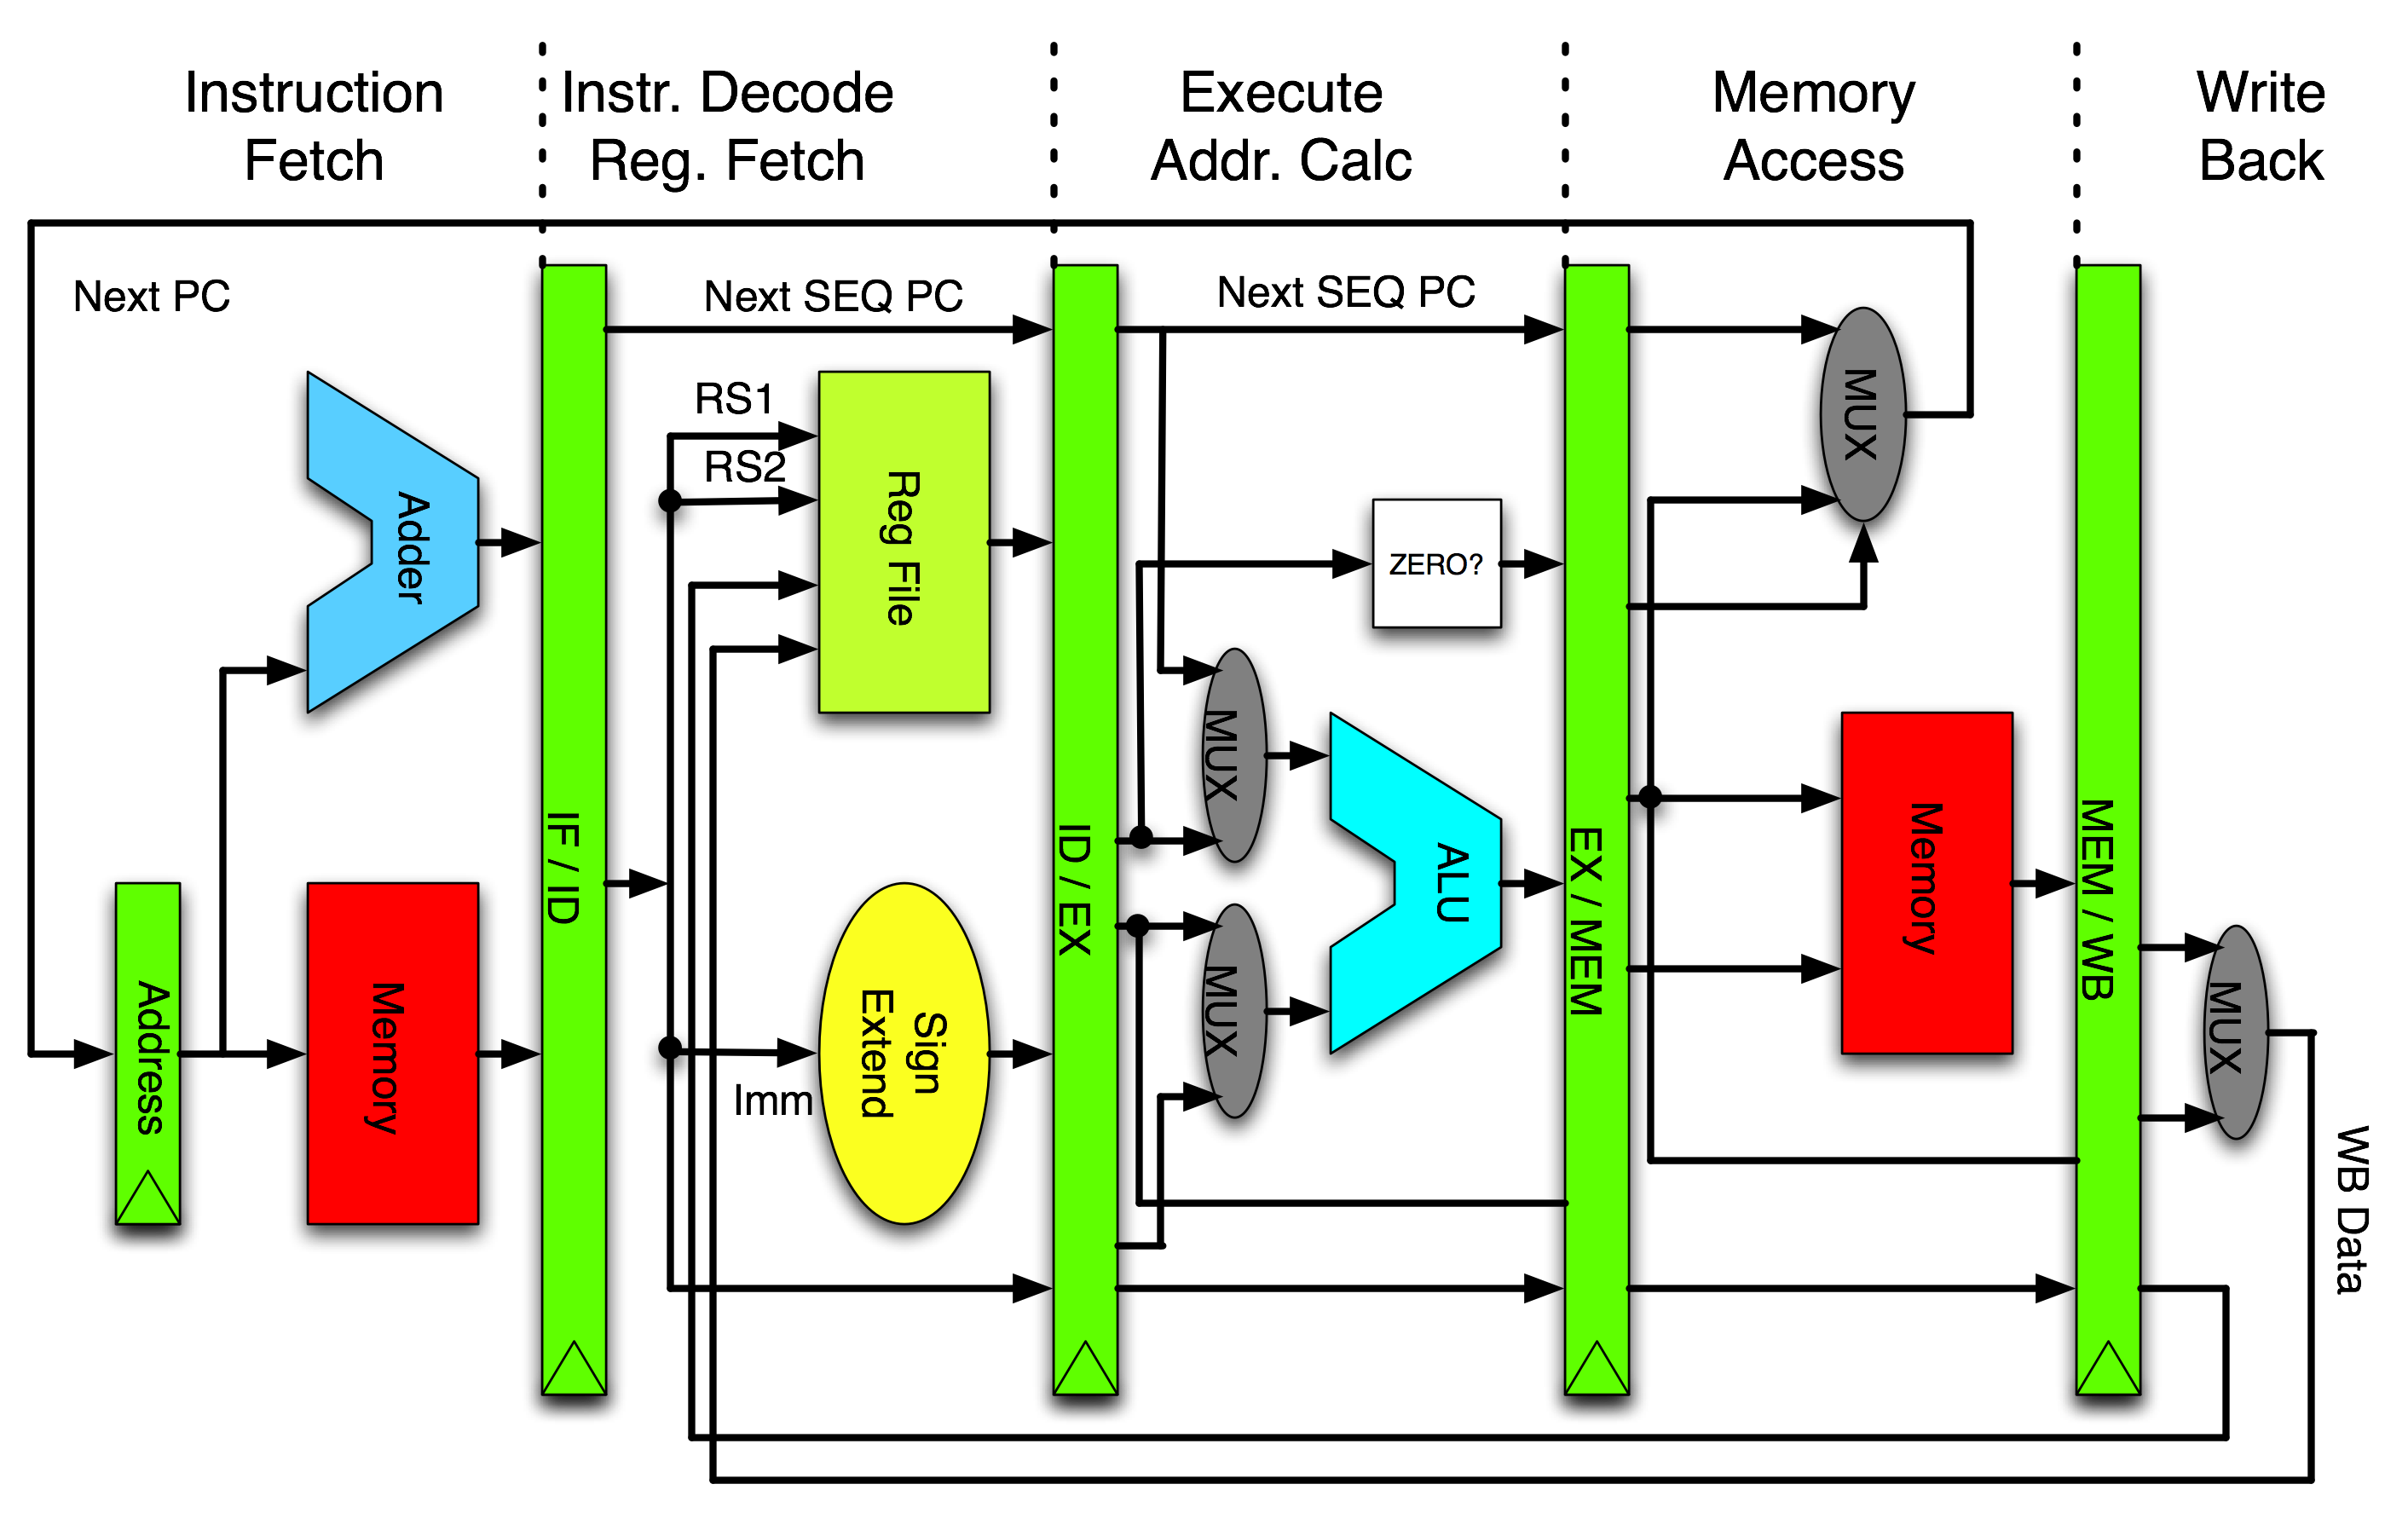
\includegraphics[width=\textwidth]{mips-pipeline.png}

  \small (MIPS, 110,000 transistors)
\end{frame}

\begin{frame}{Issues with Pipelines}
  \begin{columns}
    \column{0.5\textwidth}
      Pipelines generally help performance--but not always.

      \medskip
      Possible issue: Dependencies\dots
      \begin{itemize}
        \item \dots on memory
        \item \dots on previous computation
        \item \dots on branch outcomes
      \end{itemize}
      ``Solution'': Bubbling
    \column{0.5\textwidth}
      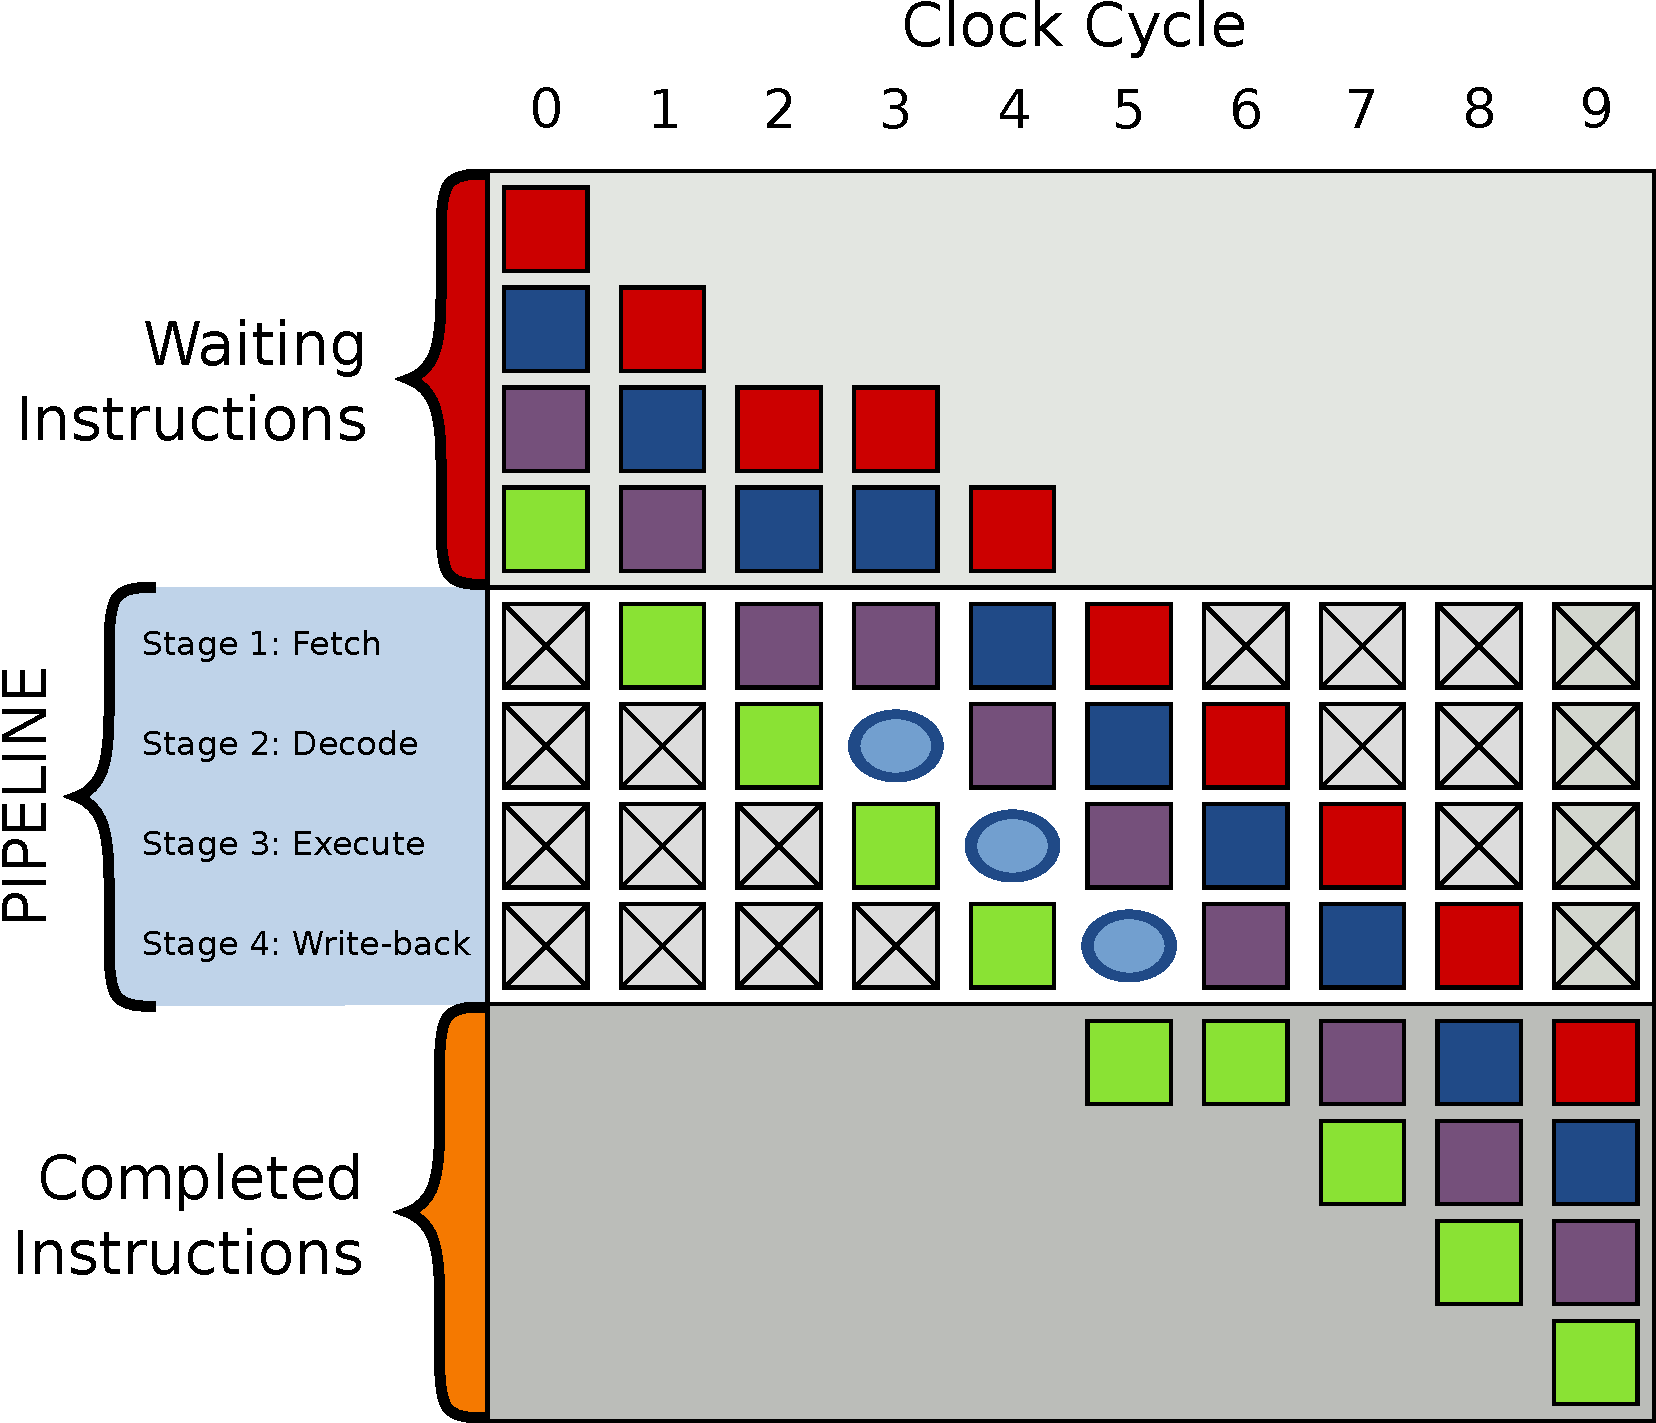
\includegraphics[width=0.8\textwidth]{pipeline-bubble.pdf}
  \end{columns}
  \uncover<2>{
    \begin{tikzpicture} [overlay]
      \node [draw,drop shadow,fill=white,anchor=south east,xshift=-0.5cm,yshift=0.5cm,
       inner sep=5mm,thick]
        at (current page.south east)
        {
          For branches: could guess\dots?
        } ;
    \end{tikzpicture}
  }
\end{frame}
\addimgcredit{Bubbly Pipeline: Wikipedia \cc}
% -----------------------------------------------------------------------------
\begin{frame}{Pipelines}
  \begin{center}
  \Huge Performance mystery demo time
  \end{center}
\end{frame}
% -----------------------------------------------------------------------------
\begin{frame}{Sandy Bridge Pipeline}
  \begin{center}
  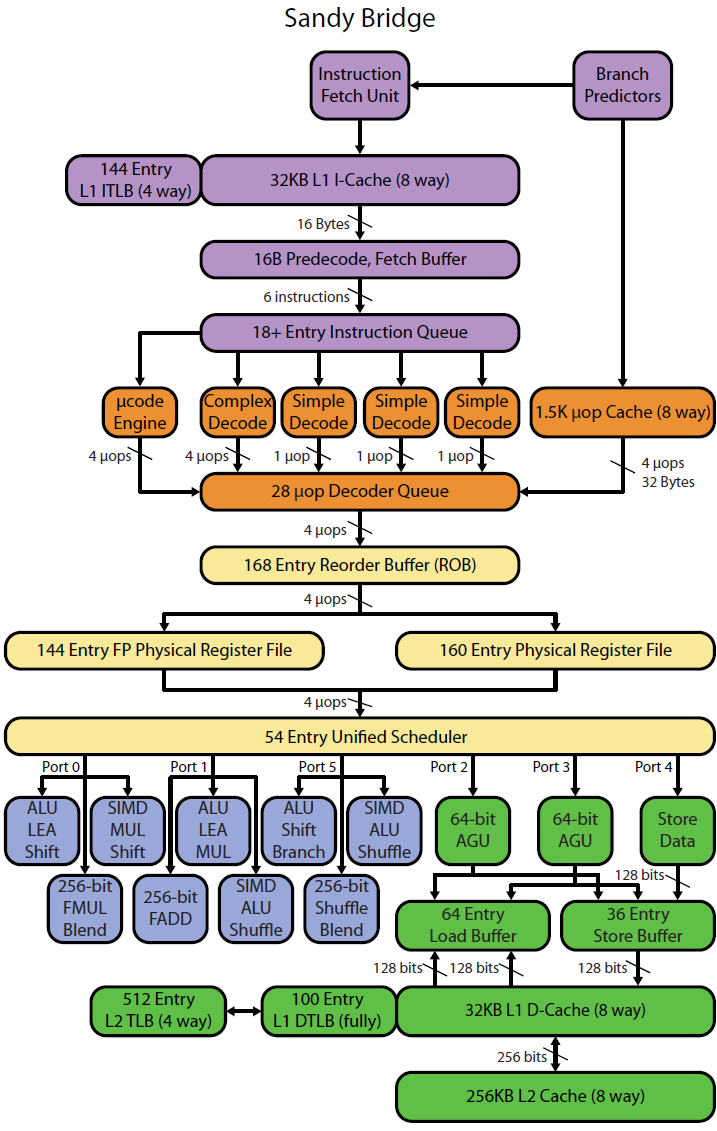
\includegraphics[height=0.85\textheight]{sandy-bridge-pipeline.png}
  \end{center}

  \creditto{David Kanter / Realworldtech.com}
  \uncover<2>{
    \begin{tikzpicture} [overlay]
      \node [draw,drop shadow,fill=white,anchor=north east,xshift=-0.5cm,yshift=-0.5cm,
      text width=0.4\textwidth, inner sep=3mm,thick]
        at (current page.north east)
        {
        New concept:\\
        Instruction-level\\
        parallelism\\
        (``Superscalar'')
        } ;
    \end{tikzpicture}
  }
\end{frame}
% -----------------------------------------------------------------------------
\begin{frame}{Pipelines}
  \begin{center}
  \Huge More Pipeline Mysteries
  \end{center}
\end{frame}
% -----------------------------------------------------------------------------
\subsection{How about actually doing work?}
% -----------------------------------------------------------------------------
{
\newcommand{\kayvoncredit}{
  \begin{tikzpicture}[overlay]
    \node [xshift=1cm,yshift=0.5cm]
      at (current page.south west)
      [font=\scriptsize,fill=gray!30,anchor=south west,opacity=0.5]
      {Credit: Kayvon Fatahalian (Stanford) };
  \end{tikzpicture}
}
\newcommand{\kayvonframe}[5]{

  \begin{frame}{#1}
    #4
    \begin{center}
    \includegraphics[viewport=#3,clip=true,page=#2,height=0.7\textheight]{kayvon-gpuarch.pdf}
    \end{center}
    \kayvoncredit
    #5
  \end{frame}
}
\begin{frame}{Remember SIMD?}
  \begin{columns}
    \column{0.5\textwidth}
      \only<1-2>{%
      \includegraphics[viewport=1.8in 3.8in 5.45in 6.25in,clip=true,page=19,width=\textwidth]{kayvon-gpuarch.pdf}\\[-0.5mm]
      \includegraphics[viewport=1.8in 1.35in 5.45in 3.8in,clip=true,page=19,width=\textwidth]{kayvon-gpuarch.pdf}
      }%
      \only<3>{%
      \includegraphics[viewport=1.8in 3.8in 5.45in 6.25in,clip=true,page=20,width=\textwidth]{kayvon-gpuarch.pdf}\\[-0.5mm]
      \includegraphics[viewport=1.8in 1.35in 5.45in 3.8in,clip=true,page=19,width=\textwidth]{kayvon-gpuarch.pdf}
      }%
      \only<4->{%
      \includegraphics[viewport=1.8in 3.8in 5.45in 6.25in,clip=true,page=20,width=\textwidth]{kayvon-gpuarch.pdf}\\[-0.5mm]
      \includegraphics[viewport=1.8in 1.35in 5.45in 3.8in,clip=true,page=20,width=\textwidth]{kayvon-gpuarch.pdf}
      }
    \column{0.5\textwidth}%
      \uncover<2->{%
        \textbf{GPU Idea \#2}

        \medskip
        Amortize cost/complexity of managing an instruction
        stream across many ALUs

        \medskip
        \large \textbf{$\rightarrow$ SIMD}
      }
  \end{columns}
  \kayvoncredit
  \uncover<2>{
    \begin{tikzpicture} [overlay]
      \node [above left=1cm of current page.south east,draw,drop shadow,fill=white,
       inner sep=5mm,thick]
        {
          Same principle works well on CPUs, too!
        } ;
    \end{tikzpicture}
  }
\end{frame}
}
% -----------------------------------------------------------------------------
\begin{frame}{Talking to SIMD}
  Ways of expressing SIMD:
  \begin{itemize}
    \item Not at all (\texttt{-ftree-vectorizer-verbose=2}, pray)
    \item ``Implicit'' (OpenCL workgroups)
    \item ``Explicit'' (many ways)
  \end{itemize}

  \bigskip
  OpenCL is also one of the saner ways of expressing
  \emph{explicit} vectorization.

  \emph{(even on the CPU)}

  \bigskip
  Other ways:
  \begin{itemize}
    \item ``Intrinsics'': \texttt{\_mm256\_hadd\_ps}
    \item GCC extensions
    \item \weblink{https://github.com/ispc/ispc}{ispc}
  \end{itemize}
\end{frame}
% -----------------------------------------------------------------------------
\begin{frame}{Floating point}
  \begin{center}
  \Huge CL vector demo
  \end{center}
\end{frame}
% -----------------------------------------------------------------------------
\begin{frame}{Floating point}
  \begin{center}
  \Huge Floating point performance demo
  \end{center}
\end{frame}
% }}}
% -----------------------------------------------------------------------------
\subsection[Compilers]{Compilers and what they do to your code}
% -----------------------------------------------------------------------------
\begin{frame}{Inside a compiler}
  \begin{center}
  \begin{tikzpicture}
  [every node/.style={draw,thick,fill=green!30,on chain,join,
  minimum height=4ex, minimum width=4cm},
  every join/.style={thick,->},
  chain default direction=going below,
  node distance=3mm,
  start chain
  ]
  \node {Preprocessor};
  \node {Parser};
  \node {\textbf<2->{Code generator}};
  \node {Assembler};
  \node {Linker};
  \node {(Dynamic Linker)};
  \end{tikzpicture}
  \end{center}
  \uncover<3->{
    \begin{tikzpicture} [overlay]
      \node [above left=1cm of current page.south east,draw,drop shadow,fill=white,
       inner sep=5mm,thick,text width=0.5\textwidth]
        {
          Two subsequent stages agree upon a data exchange format

          \bigskip
          ``Intermediate Representation''--
          often a little like assembly

          \bigskip
          Almost always more complicated: ``Passes'' include
          optimizers, etc.
        } ;
    \end{tikzpicture}
  }
\end{frame}
% -----------------------------------------------------------------------------
\begin{frame}{Compilers and the register file}
  \begin{columns}
    \column{0.6\textwidth}
      Register allocator:
      \begin{itemize}
        \item Important
        \item Complicated
      \end{itemize}

      \medskip
      Failure: `Register Spill'

      \medskip
      Not dramatic on the CPU
      (L1 is fast)

      \medskip
      \emph{Very} dramatic on the GPU
    \column{0.4\textwidth}
    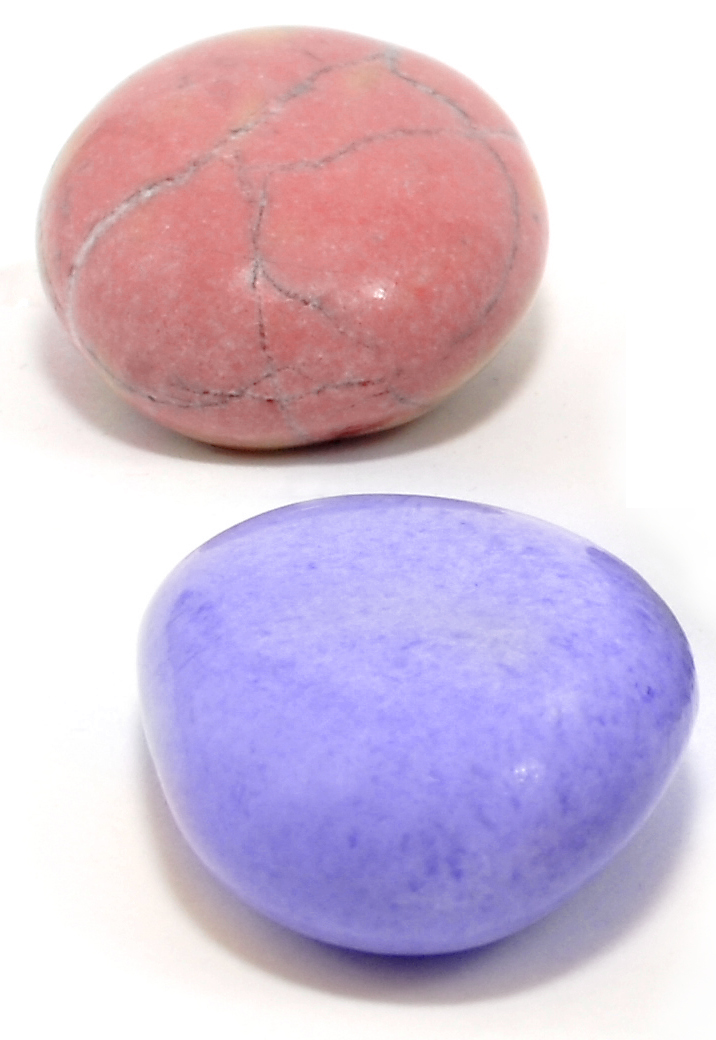
\includegraphics[width=\textwidth]{red-blue-pebble.jpeg}
  \end{columns}
  \uncover<2->{
    \begin{tikzpicture} [overlay]
      \node [above left=1cm of current page.south east,draw,drop shadow,fill=white,
       inner sep=5mm,thick]
        {
          Demo
        } ;
    \end{tikzpicture}
  }
\end{frame}
\addimgcredit{Pebbles: sxc.hu/topfer}
% -----------------------------------------------------------------------------
\begin{frame}{Pointer aliasing}
  \begin{center}
  \Huge Pointer aliasing demo
  \end{center}
\end{frame}
% -----------------------------------------------------------------------------
\begin{frame}{Alignment}
  \begin{columns}
    \column{0.45\textwidth}
    Match base address of:
    \begin{itemize}
      \item Single word: \texttt{double}, \texttt{float}
      \item SIMD vector
      \item Larger structure
    \end{itemize}
    \column{0.45\textwidth}
    To:
    \begin{itemize}
      \item Natural word size
      \item Vector size
      \item Cache line
    \end{itemize}
  \end{columns}

  \bigskip
  \begin{tikzpicture}[
    explanation/.style={right,inner xsep=0,text width=10cm}
    ]
    \foreach\addr in {0,1,...,34}
      \draw [fill=orange] 
        (0.25*\addr,0) coordinate (c\addr)
        rectangle +(0.25,0.25)
       coordinate [pos=0.5] (a\addr) ; 
    \draw (0.25*35,0) rectangle +(0.75,0.25)
       node [pos=0.5] { $\cdots$ }; 

    \foreach\addr in {0,16,32}
      \draw [ultra thick] (c\addr) -- +(0,0.25);

    \uncover<+->{
    \draw [snake=brace,thick,red] ($(c0) + (0,0.35)$) -- ($(c16) +(0,0.35)$) 
      node [pos=0.5,above] {Matched structure};
    }

    \coordinate (expl) at (0,-2.5) ;

    \uncover<+->{
      \begin{scope}[xshift=0cm,yshift=-1.5cm]
        \foreach\thread in {0,1,...,15}
          \draw [fill=gray!30] (0.25*\thread,0) rectangle +(0.25,0.25)
           coordinate [pos=0.5] (t\thread) ; 
      \end{scope}
    }

    \uncover<+>{
      \foreach\i in {0,1,...,15}
        \draw [thick,->] (t\i) -- (a\i) ;
      \node [explanation] at (expl)
      {
        {\color{green}OK}
      } ;
    }

    \uncover<+>{
      \node [explanation] at (expl)
      {
        {\color{red}``Bad''}
      } ;
    }

    \uncover<.>{
      \foreach\i in {0,1,...,15}
      {
        \pgfmathtruncatemacro{\addr}{5+\i}
        \draw [thick,->] (t\i) -- (a\addr) ;
      }
    }

    \uncover<+>{
      \foreach\i in {0,1,...,10}
      {
        \pgfmathtruncatemacro{\addr}{5+\i}
        \draw [thick,->] (t\i) -- (a\addr) ;
      }
      \foreach\i in {11,12,...,15}
      {
        \pgfmathtruncatemacro{\addr}{5+\i}
        \draw [thick,->,opacity=.1] (t\i) -- (a\addr) ;
      }
    }
    \uncover<+>{
      \foreach\i in {0,1,...,10}
      {
        \pgfmathtruncatemacro{\addr}{5+\i}
        \draw [thick,->,opacity=.1] (t\i) -- (a\addr) ;
      }
      \foreach\i in {11,12,...,15}
      {
        \pgfmathtruncatemacro{\addr}{5+\i}
        \draw [thick,->] (t\i) -- (a\addr) ;
      }
    }
  \end{tikzpicture}

  \uncover<+->{
    \begin{tikzpicture} [overlay]
      \node [above left=1cm of current page.south east,draw,drop shadow,fill=white,
       inner sep=5mm,thick, text width=0.9\textwidth]
        {
          Comes in two flavors:
          \begin{itemize}
            \item Actual alignment

              \texttt{malloc} $\rightarrow$ \texttt{posix\_memalign}
            \item Compiler-known alignment

              \texttt{float \_\_attribute\_\_ ((aligned (64))) *a}
          \end{itemize}

          \only<+->{
            \bigskip
            No difference on Sandy Bridge

            \bigskip
            More difference on other machines

            (e.g. AMD Opteron)
          }

          \only<+->{
            \bigskip
            Brief demo
          }
        } ;
    \end{tikzpicture}
  }
\end{frame}
% -----------------------------------------------------------------------------
\begin{frame}{Other compiler optimizations}
  More techniques:
  \begin{itemize}
    \item Inlining (see HW6)
    \item Unrolling
    \item Vectorization
  \end{itemize}

  \bigskip
  Many of these need tunable parameters. From where?
  \begin{itemize}
    \item \texttt{-march=native -mtune=native}
    \item Profile-Guided Optimization
  \end{itemize}
\end{frame}
% -----------------------------------------------------------------------------
\begin{frame}{From the horses' mouth}
  \begin{itemize}
    \item
      \weblink{http://support.amd.com/us/Processor_TechDocs/47414_15h_sw_opt_guide.pdf}{AMD Optimization Manual}
      \begin{itemize}
        \item Good source-level C part at the beginning
      \end{itemize}
    \item \weblink{http://www.intel.com/content/dam/doc/manual/64-ia-32-architectures-optimization-manual.pdf}{Intel Optimization Manual}
      \begin{itemize}
        \item Dual audience: Compiler writers, users
      \end{itemize}
  \end{itemize}

  \bigskip
  Grab bag of good practices:
  \begin{itemize}
    \item Use indices rather than pointers (easier to reason about)
    \item Extract common subexpressions
    \item Make functions static
    \item Use \texttt{const}
    \item Avoid store-to-load dependencies
  \end{itemize}
\end{frame}
% -----------------------------------------------------------------------------
\section{Multi-thread performance}
% -----------------------------------------------------------------------------
% {{{
\begin{frame}{Multi-thread performance}
  \begin{columns}
    \column{0.7\textwidth}

      Difference to single-thread?
      \pause

      \bigskip
      \textbf{Memory System} is (about) the only shared resource.

      \bigskip
      All `interesting' performance behavior of multiple threads
      has to do with that.
    \column{0.3\textwidth}
      \includegraphics[width=\textwidth]{memory.png}
  \end{columns}
\end{frame}
% -----------------------------------------------------------------------------
\begin{frame}{Multiple threads}
  \begin{center}
  \Huge Threads v. caches demo
  \end{center}
\end{frame}
% -----------------------------------------------------------------------------
\begin{frame}{How about multiple sockets?}
  \begin{center}
    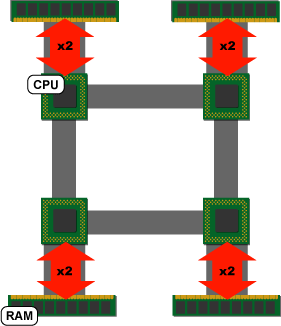
\includegraphics[height=5cm]{quad-opteron-numa.png}
  \end{center}
  \creditto{arstechnica.com}
  \uncover<+->{}
  \uncover<+->{
    \begin{tikzpicture} [overlay]
      \node [above left=1cm of current page.south east,draw,drop shadow,fill=white,
       inner sep=5mm,thick]
        {
          ``NUMA''
        } ;
    \end{tikzpicture}
  }
\end{frame}
% -----------------------------------------------------------------------------
\begin{frame}{NUMA demo}
  \begin{center}
  \Huge Contention/throughput demo
  \end{center}
\end{frame}
% -----------------------------------------------------------------------------
\begin{frame}[fragile]{NUMA results}
  \texttt{`crunchy3'} at Courant

  \medskip
  \begin{lstlisting}
    num cpus: 32
    numa available: 0
    numa node 0 10001000100010000000000000000000 - 15.9904 GiB
    numa node 1 00000000000000001000100010001000 - 16 GiB
    numa node 2 00010001000100010000000000000000 - 16 GiB
    numa node 3 00000000000000000001000100010001 - 16 GiB
    numa node 4 00100010001000100000000000000000 - 16 GiB
    numa node 5 00000000000000000010001000100010 - 16 GiB
    numa node 6 01000100010001000000000000000000 - 16 GiB
    numa node 7 00000000000000000100010001000100 - 16 GiB
  \end{lstlisting}
\end{frame}
% -----------------------------------------------------------------------------
\begin{frame}[fragile]{NUMA results}
  \texttt{`crunchy3'} at Courant

  \medskip
  \begin{lstlisting}
    sequential core 0 -> core 0 : BW 4189.87 MB/s
    sequential core 1 -> core 0 : BW 2409.1 MB/s
    sequential core 2 -> core 0 : BW 2495.61 MB/s
    sequential core 3 -> core 0 : BW 2474.62 MB/s
    sequential core 4 -> core 0 : BW 4244.45 MB/s
    sequential core 5 -> core 0 : BW 2378.34 MB/s
    ....
    sequential core 29 -> core 0 : BW 2048.68 MB/s
    sequential core 30 -> core 0 : BW 2087.6 MB/s
    sequential core 31 -> core 0 : BW 2014.68 MB/s
  \end{lstlisting}
\end{frame}
% -----------------------------------------------------------------------------
\begin{frame}[fragile]{NUMA results}
  \texttt{`crunchy3'} at Courant

  \medskip
  \begin{lstlisting}
    all-contention core 0 -> core 0 : BW 1081.85 MB/s
    all-contention core 1 -> core 0 : BW 299.177 MB/s
    all-contention core 2 -> core 0 : BW 298.853 MB/s
    all-contention core 3 -> core 0 : BW 263.735 MB/s
    all-contention core 4 -> core 0 : BW 1081.93 MB/s
    all-contention core 5 -> core 0 : BW 299.177 MB/s
    ....
    all-contention core 27 -> core 0 : BW 202.49 MB/s
    all-contention core 28 -> core 0 : BW 434.295 MB/s
    all-contention core 29 -> core 0 : BW 233.309 MB/s
    all-contention core 30 -> core 0 : BW 233.169 MB/s
    all-contention core 31 -> core 0 : BW 202.526 MB/s
  \end{lstlisting}
\end{frame}
% -----------------------------------------------------------------------------
\begin{frame}[fragile]{NUMA results}
  \texttt{`crunchy3'} at Courant

  \medskip
  \begin{lstlisting}
    two-contention core 0 -> core 0 : BW 3306.11 MB/s
    two-contention core 1 -> core 0 : BW 2199.7 MB/s

    two-contention core 0 -> core 0 : BW 3257.56 MB/s
    two-contention core 19 -> core 0 : BW 1885.03 MB/s
  \end{lstlisting}
\end{frame}
% }}}
% -----------------------------------------------------------------------------
%\section{GPU performance}
% -----------------------------------------------------------------------------
% {{{
% - Local memory
%   - Bank conflicts
% - Global memory (AMD!)
%   - Soa vs Aos
%   - Coalescing
%   - Caches
%   - Partition camping
% - Memory zoo
% - Register file
%   - Cost of spills
% - Occupancy
% - ILP vs other forms of parallelism
% }}}


\questionframe{}
\imagecreditslide

\end{document}
% vim: foldmethod=marker
